% ============================================================================
% NLOS Detection and Weighted Multilateration
% ============================================================================

\subsection{Non-Line-of-Sight: Causes and Impact}
\label{sec:nlos_background}

A \emph{line-of-sight} (LOS) UWB link exists when there is an unobstructed
straight-line path between transmitter and receiver.
\emph{Non-line-of-sight} (NLOS) arises when this path is blocked or
heavily diffracted, so the first received signal has travelled a longer
route than the geometric distance.
Four mechanisms are relevant in our deployment:
\textit{hard blocking} by the rover's chassis or manipulator arm;
\textit{soft blocking} by wooden partitions or sandbags;
\textit{dynamic obstruction} as the arm swings or the rover rotates;
and \textit{grazing incidence} near the sandy floor.

Because ToA-based ranging locks onto the first arriving pulse, NLOS adds
an always-positive bias $\Delta_i \geq 0$ to the measured range:
\begin{equation}
  \rho_i^{\text{NLOS}} = \|\mathbf{p} - \mathbf{a}_i\| + \Delta_i + \varepsilon_i,
  \label{eq:nlos_range}
\end{equation}
with $\Delta_i \in [0.02,\,0.50]$\,m in practice.
From the Jacobian structure~\eqref{eq:jacobian}, a bias $\Delta_i$ on anchor~$i$
shifts the estimated position by
$\|\delta\hat{\mathbf{p}}\| \approx \Delta_i\,\|(\mathbf{J}^\top\mathbf{J})^{-1}
\mathbf{j}_i\|$, which can exceed $\Delta_i$ for unfavourable geometries.
Crucially, this is a \emph{systematic bias}, not noise: it cannot be averaged
away, and it worsens as the rover moves toward the obstruction.

\subsection{Same-Frame NLOS Detection}

\begin{figure}[t]
  \centering
  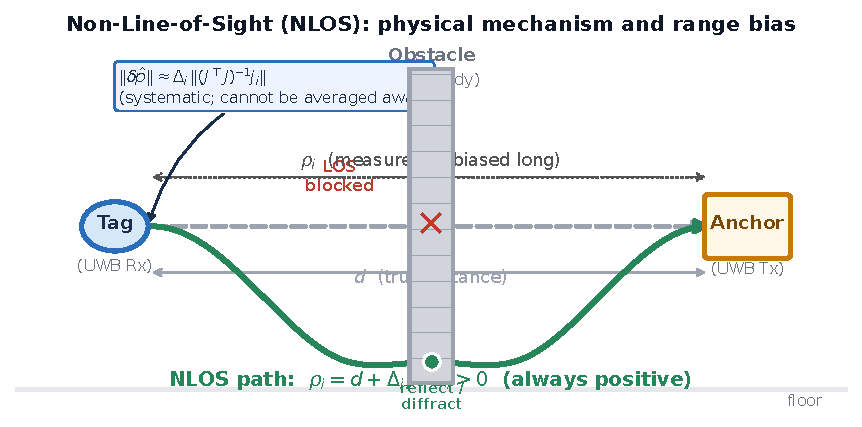
\includegraphics[width=\columnwidth]{figures/nlos_concept.pdf}
  \caption{Physical NLOS scenario.
  The direct LOS path is blocked by an obstacle; the signal arrives via a
  longer reflected or diffracted route, adding always-positive range bias
  $\Delta_i > 0$ to the measured range $\rho_i = d + \Delta_i$.
  Because ToA locks on the first arriving pulse, the bias is systematic ---
  it cannot be averaged away and worsens as the rover approaches the obstruction.
  The position error $\|\delta\hat{\mathbf{p}}\|\approx\Delta_i\|(\mathbf{J}^\top\mathbf{J})^{-1}\mathbf{j}_i\|$
  can exceed $\Delta_i$ under poor anchor geometry.}
  \label{fig:nlos_concept}
\end{figure}

The DW1000 channel impulse response exposes two power registers per received
frame: total received power $P_\text{rx}$ and first-path power $P_\text{fp}$.
Under LOS, $P_\text{rx} \approx P_\text{fp}$; under NLOS, reflected paths
dominate while the direct path is attenuated, so $P_\text{rx} > P_\text{fp}$.
The gap \cite{aps006} is:
\begin{align}
  P_{\text{fp}} &= 10\log_{10}\!\Bigl(\frac{F_1^2+F_2^2+F_3^2}{N^2}\Bigr) - 115.72
  \label{eq:fp_power}\\
  \text{gap}_i &= P_{\text{rx},i} - P_{\text{fp},i},
  \label{eq:nlos_gap}
\end{align}
where $F_1,F_2,F_3$ are first-path amplitude registers and $N$ is the
preamble accumulation count.

\textbf{Prior implementation error.}
Existing DW1000 libraries read $P_\text{rx}$ from one link and $P_\text{fp}$
from a \emph{different} link, making the gap physically meaningless:
the anchor-to-tag channel can be LOS while the tag-to-anchor channel is
NLOS, or vice versa.

\textbf{Our fix.}
We read both $P_\text{rx}$ and $P_\text{fp}$ from the \emph{same}
RANGE\_REPORT frame on the \emph{tag side}, immediately after reception.
This yields a valid same-link indicator.
We classify: LOS if $\text{gap}_i < 3\,\text{dB}$;
soft NLOS if $3 \leq \text{gap}_i < 6\,\text{dB}$;
hard NLOS if $\text{gap}_i \geq 6\,\text{dB}$.

\subsection{Robust Weighted Multilateration}

\begin{figure}[h]
  \centering
  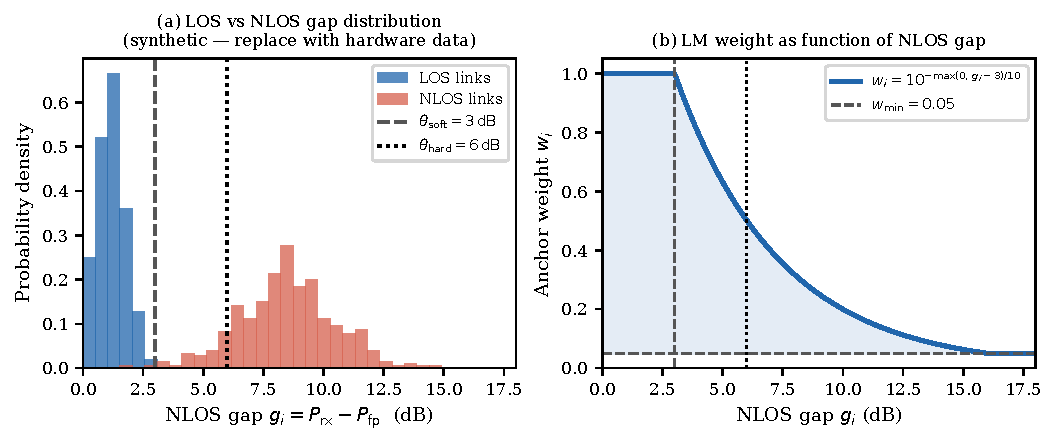
\includegraphics[width=\columnwidth]{figures/nlos_diagram.pdf}
  \caption{\textit{(a)}~NLOS gap distribution under LOS and obstructed
  conditions (synthetic placeholder).
  \textit{(b)}~Per-anchor LM weight as a function of gap; soft threshold
  $\theta_\text{soft}=3\,\mathrm{dB}$, floor $w_{\min}=0.05$.}
  \label{fig:nlos_gap}
\end{figure}

We solve~\eqref{eq:multilateration} via weighted Levenberg--Marquardt.
The per-anchor weight derived from the NLOS gap is:
\begin{equation}
  w_i = \max\Bigl(w_{\min},\;
        10^{-\max(0,\,\text{gap}_i - 3)/10}\Bigr),
  \label{eq:nlos_weight}
\end{equation}
with $w_{\min} = 0.05$ (Fig.~\ref{fig:nlos_gap}b).
A 10\,dB gap gives $w_i = 0.10$ --- the anchor contributes one-tenth
the influence of a clean LOS measurement.
The output covariance~\eqref{eq:lm_cov} propagates this weighting into the
EKF, so down-weighted fixes report larger position uncertainty.

\textbf{MAD outlier gate.}
Independent of soft weighting, we apply a gross-outlier gate after a first
LM pass: anchor~$i$ is rejected if
$|r_i - \mathrm{median}(\mathbf{r})| > 3.0 \times 1.4826 \times \mathrm{MAD}(\mathbf{r})$.
A second LM solve runs on the retained set.
The MAD gate handles catastrophic outliers; the NLOS weighting handles
consistent sub-catastrophic bias --- two independent, complementary defences.

\textbf{Range bias correction.}
A first-order range correction
$\rho_i^\text{corr} = \rho_i - k_\text{NLOS}\max(0,\,\text{gap}_i - 3)$
with $k_\text{NLOS} \in [0,\,0.06]$\,m/dB is available but disabled by
default until the gap-to-path-length relationship is characterised for
the specific deployment.
\todo{Characterise $k_\text{NLOS}$ from a through-wall NLOS experiment.}
